% Made up for the tikra benchmark.
\usetikzlibrary{fadings}
\begin{tikzfadingfrompicture}[name=fade right]
  \shade[left color=transparent!0, right color=transparent!90] (-4,-2.2) rectangle (4,2.2);
\end{tikzfadingfrompicture}
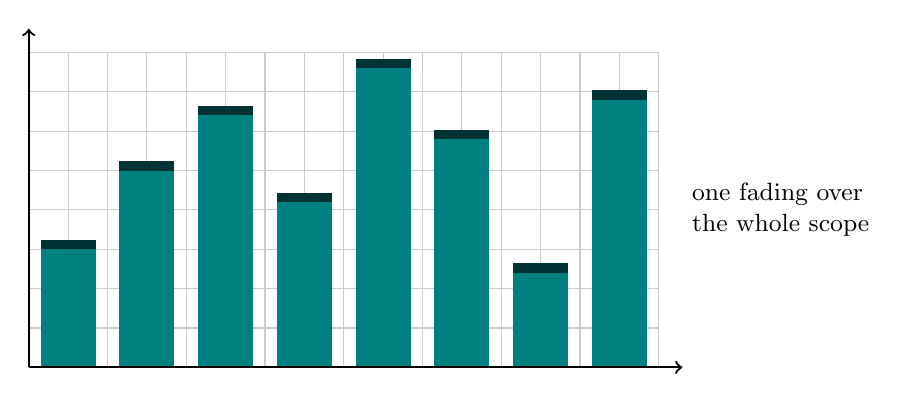
\begin{tikzpicture}
  \draw[gray!40] (-4,-2) grid[step=0.5] (4,2);
  \begin{scope}[scope fading=fade right]
    \foreach \h [count=\i from -4] in {1.5,2.5,3.2,2.1,3.8,2.9,1.2,3.4} {
      \fill[teal] (\i+0.15,-2) rectangle +(0.7,\h);
      \fill[teal!40!black] (\i+0.15,\h-2) rectangle +(0.7,0.12);
    }
  \end{scope}
  \draw[thick, ->] (-4,-2) -- (4.3,-2);
  \draw[thick, ->] (-4,-2) -- (-4,2.3);
  \node[anchor=west, font=\small, align=left] at (4.3,0) {one fading over\\the whole scope};
\end{tikzpicture}
